\documentclass[11pt,a4paper]{article}
\usepackage[margin=18mm]{geometry}
\usepackage{amsmath,amssymb,mathtools}
\usepackage{booktabs,array,enumitem}
\usepackage[dvipsnames]{xcolor}
\usepackage{graphicx,listings,tikz}
\usetikzlibrary{arrows.meta,positioning}
\usepackage[most]{tcolorbox}
\usepackage{hyperref}
\usepackage{needspace}
\hypersetup{colorlinks=true,urlcolor=MidnightBlue,linkcolor=MidnightBlue}
\setlength{\parindent}{0pt}\setlength{\parskip}{4pt}
\newcommand{\course}{PHY4605 Computational Methods in Physics}
\newcommand{\units}[1]{\,\mathrm{#1}}
\newtcolorbox{keybox}{colback=RoyalBlue!5,colframe=RoyalBlue!65!black,boxrule=.7pt,arc=2mm}
\newtcolorbox{checkbox}{colback=ForestGreen!5,colframe=ForestGreen!55!black,boxrule=.7pt,arc=2mm}
\newtcolorbox{aibox}{colback=BurntOrange!7,colframe=BurntOrange!80!black,boxrule=.7pt,arc=2mm}
\lstdefinestyle{matlabstyle}{language=Matlab,basicstyle=\ttfamily\footnotesize,keywordstyle=\color{RoyalBlue!75!black},commentstyle=\color{ForestGreen!55!black},stringstyle=\color{BurntOrange!80!black},numbers=left,numberstyle=\scriptsize\color{black!50},numbersep=5pt,frame=single,rulecolor=\color{RoyalBlue!25},backgroundcolor=\color{RoyalBlue!3},showstringspaces=false,columns=fullflexible,keepspaces=true,breaklines=true}
\begin{document}
{\large\textsc{\course}}\\[-2pt]
{\small Learning Note \textbar\ Week 11}\par\vspace{4pt}
{\LARGE\bfseries Sensitivity and Uncertainty Propagation}\par\vspace{3pt}
\textit{Use controlled parameter variation to turn plausible input uncertainty into an output range that can be validated and interpreted physically.}

\begin{keybox}\textbf{Physical question.} A spring is loaded by a known force, but its stiffness is only known within a plausible range. What range of extension should we report, and what does that range say about the reliability of the prediction?\end{keybox}

\section*{Core learning outcomes}
\begin{enumerate}[nosep,leftmargin=5mm]
\item convert one uncertain input into lower, baseline, and upper one-at-a-time model evaluations;
\item report and validate the resulting output range without false precision; and
\item distinguish parameter uncertainty, numerical approximation error, and model limitation in plain language.
\end{enumerate}

\section*{1. From a parameter sweep to uncertainty evidence}
In Week 4, changing a model parameter helped reveal a physical trend. Week 11 uses the same computational move for a different purpose: the input is not known exactly, so a plausible input range becomes uncertainty evidence.

The familiar model is the ideal linear spring,
\[
F=kx, \qquad x=\frac{F}{k}.
\]
In words: for a fixed applied force, the predicted extension is the force divided by the spring stiffness. We use
\[
F=10\units{N}, \qquad k_0=100\units{N\,m^{-1}},
\]
with a plausible stiffness range from $95$ to $105\units{N\,m^{-1}}$.

\begin{center}\small
\begin{tabular}{>{\raggedright\arraybackslash}p{.20\linewidth}>{\raggedright\arraybackslash}p{.23\linewidth}>{\raggedright\arraybackslash}p{.43\linewidth}}
\toprule
Quantity & Week 11 value & Meaning \\
\midrule
$F$ & $10\units{N}$ & applied force held fixed in the Core sweep \\
$k$ & $95,100,105\units{N\,m^{-1}}$ & plausible lower, baseline, and upper stiffness values \\
$x$ & m & model output: predicted extension \\
\bottomrule
\end{tabular}
\end{center}

\begin{checkbox}\textbf{Prediction checkpoint.} Because $x=F/k$, lower stiffness should produce larger extension. The $95\units{N\,m^{-1}}$ case should therefore give the largest $x$, while the $105\units{N\,m^{-1}}$ case should give the smallest.\end{checkbox}

\section*{2. One-at-a-time uncertainty reasoning}
A one-at-a-time sweep changes one uncertain input while keeping the model and every other input fixed. This allows the resulting output change to be attributed to that one input range.

\begin{center}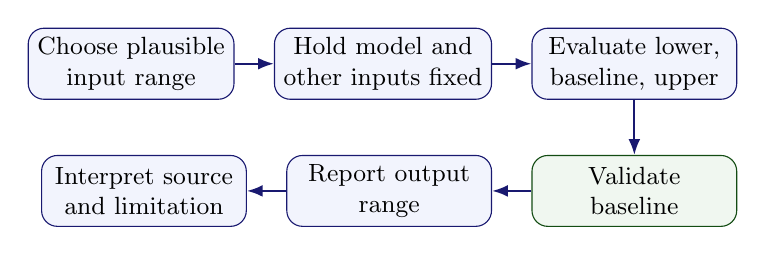
\begin{tikzpicture}[node distance=7mm and 5mm,every node/.style={font=\small,align=center},box/.style={draw=MidnightBlue,rounded corners=2mm,fill=RoyalBlue!7,minimum width=26mm,minimum height=9mm},check/.style={draw=ForestGreen!55!black,rounded corners=2mm,fill=ForestGreen!7,minimum width=26mm,minimum height=9mm},arrow/.style={-{Latex[length=2mm]},thick,MidnightBlue}]
\node[box] (r) {Choose plausible\\input range};
\node[box,right=of r] (h) {Hold model and\\other inputs fixed};
\node[box,right=of h] (e) {Evaluate lower,\\baseline, upper};
\node[check,below=of e] (v) {Validate\\baseline};
\node[box,left=of v] (o) {Report output\\range};
\node[box,left=of o] (i) {Interpret source\\and limitation};
\draw[arrow] (r)--(h); \draw[arrow] (h)--(e); \draw[arrow] (e)--(v); \draw[arrow] (v)--(o); \draw[arrow] (o)--(i);
\end{tikzpicture}\end{center}

The computational recipe is:
\begin{enumerate}[nosep,leftmargin=7mm]
\item define the model, baseline, units, and one plausible input range;
\item hold all other inputs and assumptions fixed;
\item evaluate the lower, baseline, and upper cases;
\item collect the minimum and maximum output;
\item validate one known or hand-calculated case; and
\item state what the output range means physically.
\end{enumerate}

\begin{aibox}\textbf{Do not vary several uncertain inputs at once when the question asks which input caused the change.} Simultaneous variation can be useful for other analyses, but it no longer isolates one input's effect.\end{aibox}

\section*{3. MATLAB scaffold: three controlled cases}
The Core calculation needs only a short array and element-wise division. The three stiffness values form three controlled evaluations of the same deterministic equation.

\begin{lstlisting}[style=matlabstyle]
force_baseline_N = 10;
stiffness_baseline_Npm = 100;
stiffness_cases_Npm = [95 100 105];

extension_cases_m = force_baseline_N./stiffness_cases_Npm;
extension_baseline_m = force_baseline_N/stiffness_baseline_Npm;
extension_range_m = [min(extension_cases_m) max(extension_cases_m)];
\end{lstlisting}

The dot in \texttt{./} means that the scalar force is divided by each stored stiffness value. The calculation gives
\[
x_0=0.10000\units{m},
\]
and the range
\[
0.09524\units{m}\lesssim x \lesssim 0.10526\units{m}.
\]

\begin{figure}[h]
\centering
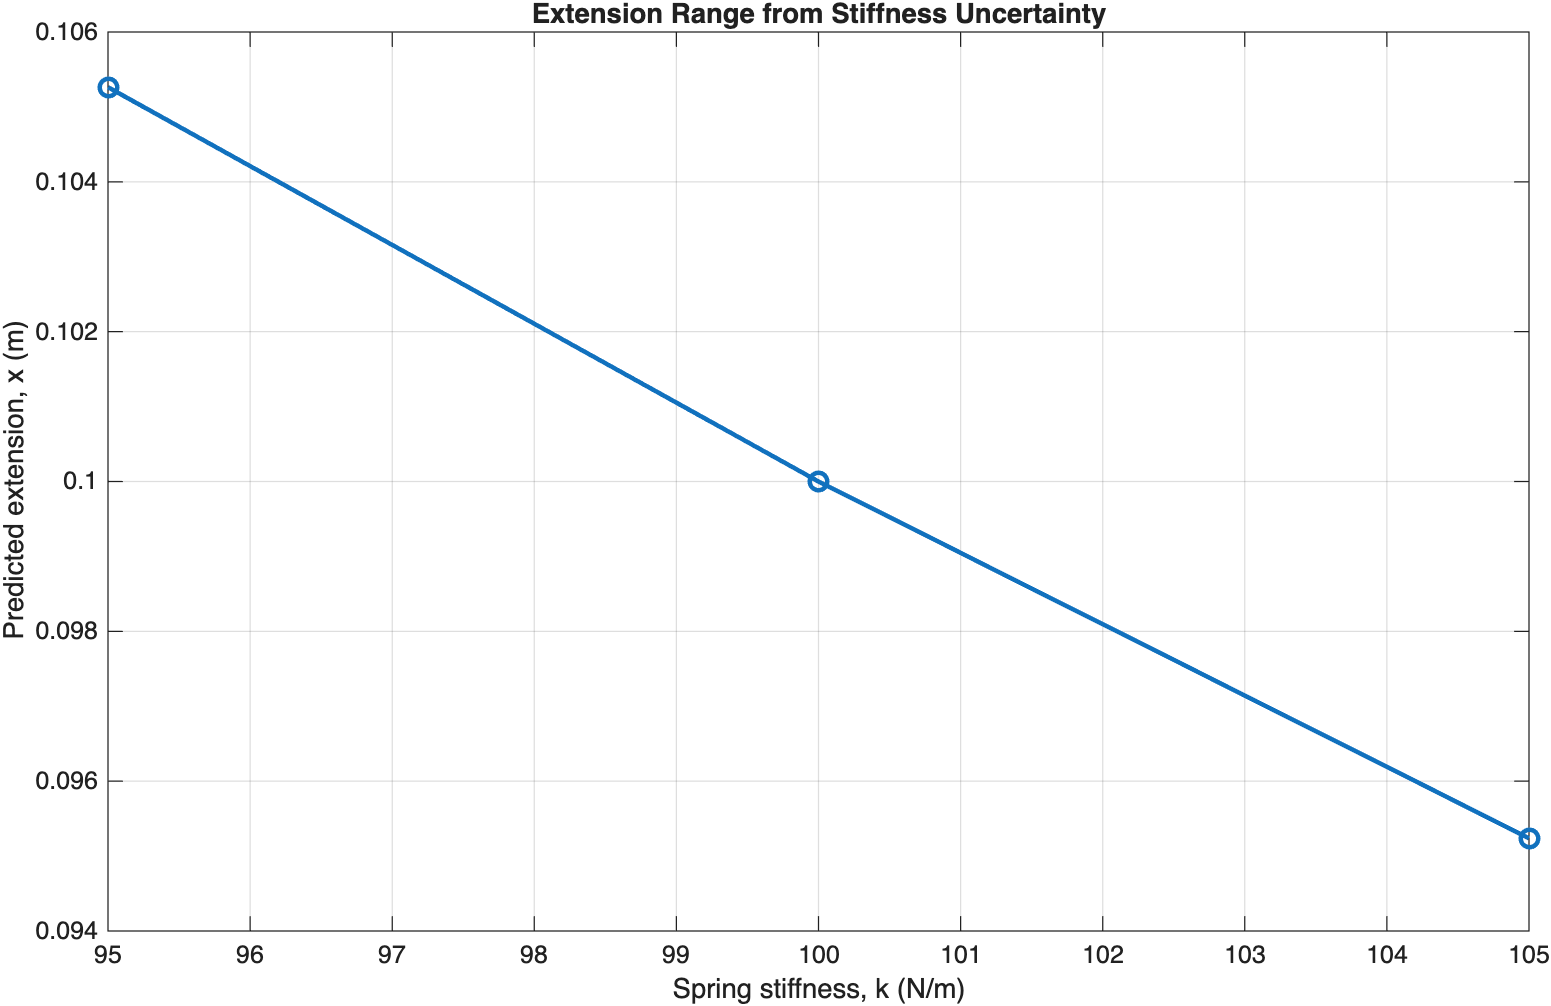
\includegraphics[width=.76\linewidth]{assets/week11_hooke_stiffness_uncertainty.png}
\caption{Predicted extension for the supplied stiffness values. These points are controlled parameter cases, not repeated random trials.}
\end{figure}

\section*{4. Report a range, not just a long decimal}
The exact-looking statement ``$x=0.10000\units{m}$'' describes only the baseline case. It hides the fact that the stiffness itself is uncertain over the supplied range.

A more defensible statement is:

\begin{keybox}\textbf{Range-based result.} For a $10\units{N}$ load and stiffness between $95$ and $105\units{N\,m^{-1}}$, the ideal Hooke model predicts an extension of about $0.095$ to $0.105\units{m}$.\end{keybox}

Extra displayed decimal places do not improve knowledge of the spring stiffness. Numerical display precision and physical parameter uncertainty are different ideas.

\section*{5. Core validation: check the baseline independently}
The baseline is simple enough to calculate by hand:
\[
x_0=\frac{10\units{N}}{100\units{N\,m^{-1}}}=0.10\units{m}.
\]
The units also reduce correctly:
\[
\frac{\mathrm{N}}{\mathrm{N\,m^{-1}}}=\mathrm{m}.
\]

\begin{lstlisting}[style=matlabstyle]
reference_baseline_m = 10/100;
baseline_check_passed = abs(extension_baseline_m-reference_baseline_m) < 1e-12;
assert(baseline_check_passed,'Baseline Hooke-law validation failed.')
\end{lstlisting}

\begin{checkbox}\textbf{Validation result.} The baseline matches the independent calculation, the units are metres, and the trend is physically consistent: decreasing $k$ increases $x$ at fixed $F$. A smooth graph alone would not establish these checks.\end{checkbox}

\section*{6. Three different reasons a prediction can be imperfect}
The word ``error'' is too vague unless its source is identified.

\begin{center}\small
\begin{tabular}{>{\raggedright\arraybackslash}p{.22\linewidth}>{\raggedright\arraybackslash}p{.34\linewidth}>{\raggedright\arraybackslash}p{.34\linewidth}}
\toprule
Source & Meaning & Week 11 example \\
\midrule
Parameter uncertainty & an input is not known exactly & spring stiffness is plausible from $95$ to $105\units{N\,m^{-1}}$ \\
Numerical approximation error & a mathematical operation is approximated numerically & a finite timestep changes an ODE simulation result \\
Model limitation & the equation's assumptions do not fully represent reality & Hooke's law may fail outside the linear elastic range \\
\bottomrule
\end{tabular}
\end{center}

The direct Core Hooke calculation has no meaningful timestep, grid, or iterative approximation. Its uncertainty range comes from the stated stiffness range. Even a perfectly evaluated equation can still inherit uncertainty from its inputs and limitations from its assumptions.

\section*{7. Worked reasoning chain}
\begin{center}\small
\begin{tabular}{p{.25\linewidth}p{.67\linewidth}}
\toprule
Step & Week 11 evidence \\
\midrule
Physical model & ideal linear spring, $x=F/k$ \\
Scale and units & $F$ in N, $k$ in N/m, $x$ in m \\
Uncertain input & $k=95,100,105\units{N\,m^{-1}}$ \\
Algorithm & hold $F$ fixed, evaluate the same model for lower/baseline/upper $k$ \\
Output range & approximately $0.09524$ to $0.10526\units{m}$ \\
Validation & hand-check $10/100=0.10\units{m}$ plus units and trend \\
Interpretation & stiffness uncertainty creates a range of plausible model predictions \\
\bottomrule
\end{tabular}
\end{center}

This chain is more important than memorising a MATLAB function name. In an assessment, syntax may be supplied; the physical model, held-fixed conditions, uncertainty source, validation, and interpretation still need to be defended.

\section*{Working exposure: compare a second uncertain input}
Now hold $k=100\units{N\,m^{-1}}$ fixed and vary the force from $9.8$ to $10.2\units{N}$. The corresponding extension range is $0.098$ to $0.102\units{m}$, with a full span of $0.004\units{m}$.

For the stiffness range, the full extension span is about $0.01003\units{m}$. For the supplied uncertainty ranges, stiffness therefore changes the output more than force. This conclusion depends on the ranges that were supplied; it is not a universal statement that stiffness must always dominate force.

\begin{figure}[h]
\centering
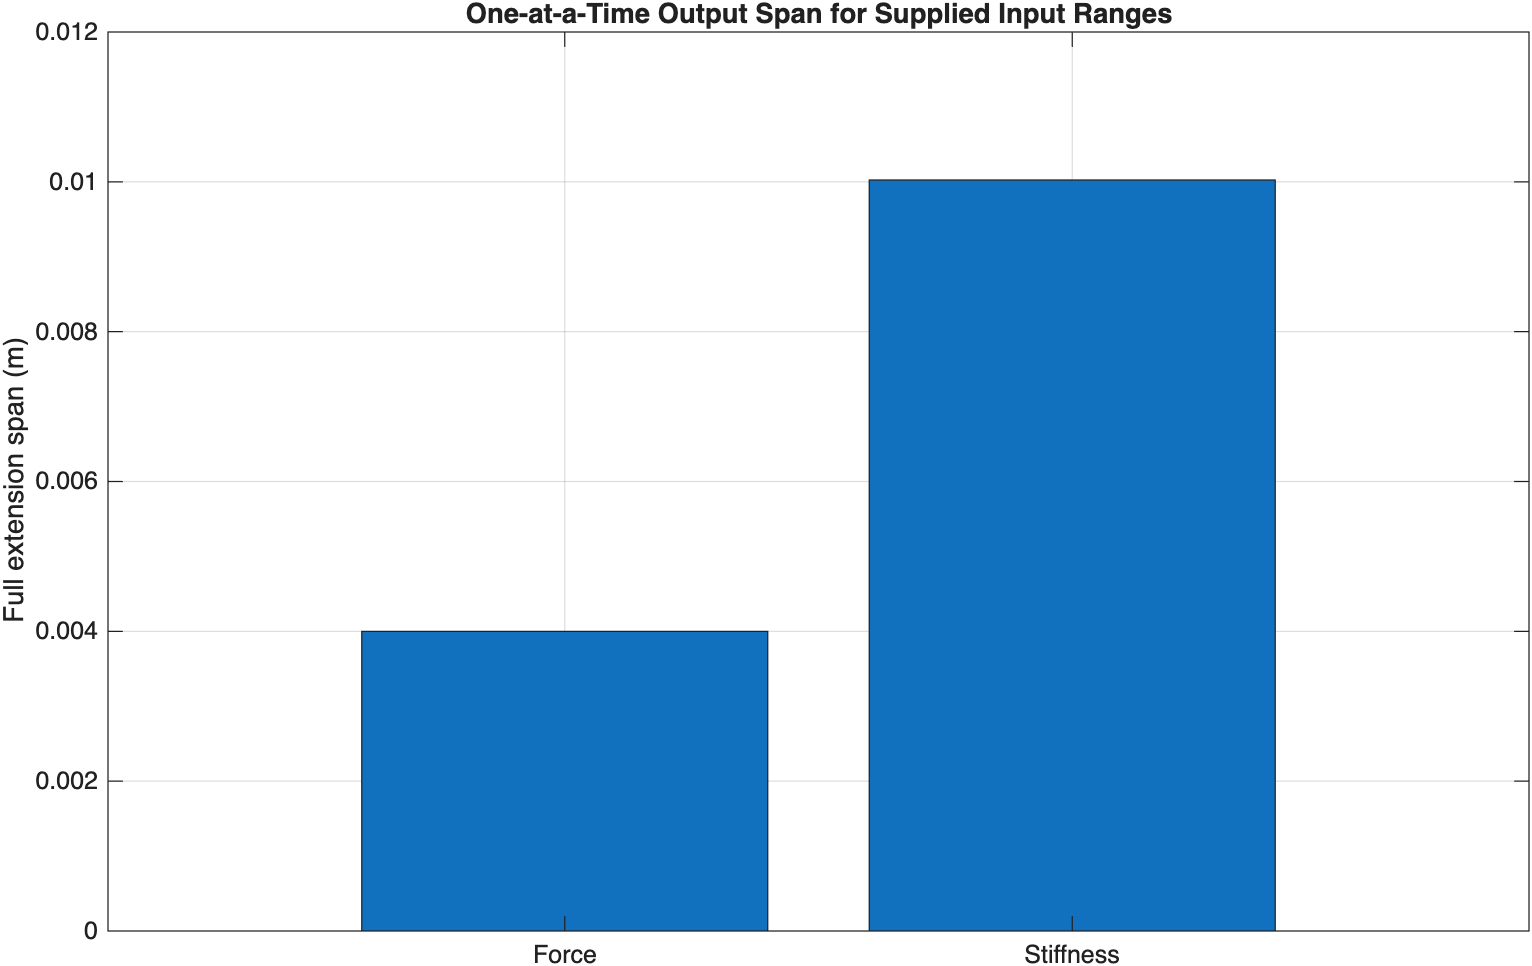
\includegraphics[width=.70\linewidth]{assets/week11_one_at_a_time_comparison.png}
\caption{One-at-a-time output spans for the supplied stiffness and force ranges. The comparison isolates one input range at a time.}
\end{figure}

\Needspace{18\baselineskip}
\section*{Working exposure: supplied sensitivity and propagation formulas}
A supplied normalized sensitivity can compare fractional output change with fractional input change near a baseline:
\[
S\approx\frac{\Delta x/x_0}{\Delta p/p_0}.
\]
For $x=F/k$, the supplied local interpretation is approximately $S_k=-1$ and $S_F=+1$. The sign gives the direction of response; the magnitude describes the fractional responsiveness near the baseline. Deriving these sensitivities is not Core Week 11 work.

If small force and stiffness uncertainties are treated as independent standard uncertainties, a supplied first-order relation is
\[
\frac{u_x}{x}\approx\sqrt{\left(\frac{u_F}{F}\right)^2+\left(\frac{u_k}{k}\right)^2}.
\]
Using $u_F=0.2\units{N}$ and $u_k=5\units{N\,m^{-1}}$ gives a relative estimate of about $5.39\%$ and
\[
u_x\approx0.00539\units{m}.
\]
This combined estimate answers a different question from the isolated one-at-a-time ranges. The formula is supplied for interpretation only.

\section*{Optional stretch}
Independent derivative-based propagation, Monte Carlo uncertainty propagation, correlated inputs, interaction effects, and global sensitivity methods are outside the Week 11 Core route.

\section*{Three takeaways}
\begin{enumerate}[nosep,leftmargin=7mm]
\item An uncertain input should be represented by a justified baseline and plausible range before evaluating the model.
\item A one-at-a-time sweep converts that input range into an interpretable output range while keeping other inputs fixed.
\item Parameter uncertainty, numerical approximation error, and model limitation describe different reasons a prediction may be imperfect.
\end{enumerate}

\begin{keybox}\textbf{Preparation for the practical.} Be ready to identify one uncertain input and its units, predict the direction of the output change, compute a lower/baseline/upper range using a supplied model, perform one independent check, and explain the result without false precision.\end{keybox}

\end{document}
